\Problem
{گام هفتم}
{
    مطابق کدی که در اسلاید‌ها بود تصویر خاکستری و نویزی را به حوزه فرکانس می‌بریم.
    
    با استفاده از دستور 
    \lr{fft2} 
    می‌توانیم عکس را از حوزه 
    \lr{Spatial} 
    به حوزه فرکانس ببریم.
    
    این دستور بر روی یک ماتریس یک تبدیل فوریه گسسته 
    \lr{DFT} 
    می‌گیرد. و رابطه آن به صورت زیر است:
    
    \begin{figure}[H]
        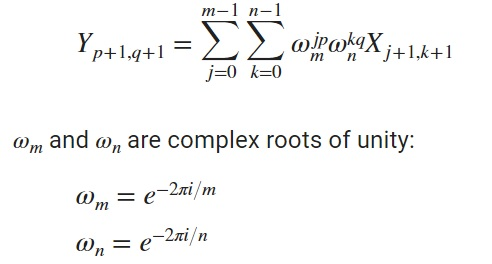
\includegraphics[]{Images/FFT2.jpg}
        \centering
        \caption{رابطه تبدیل فوریه دو بعدی}
    \end{figure}
    
    \newpage
    \begin{figure}[H]
        \centering
        \begin{minipage}[b]{0.4\textwidth}
            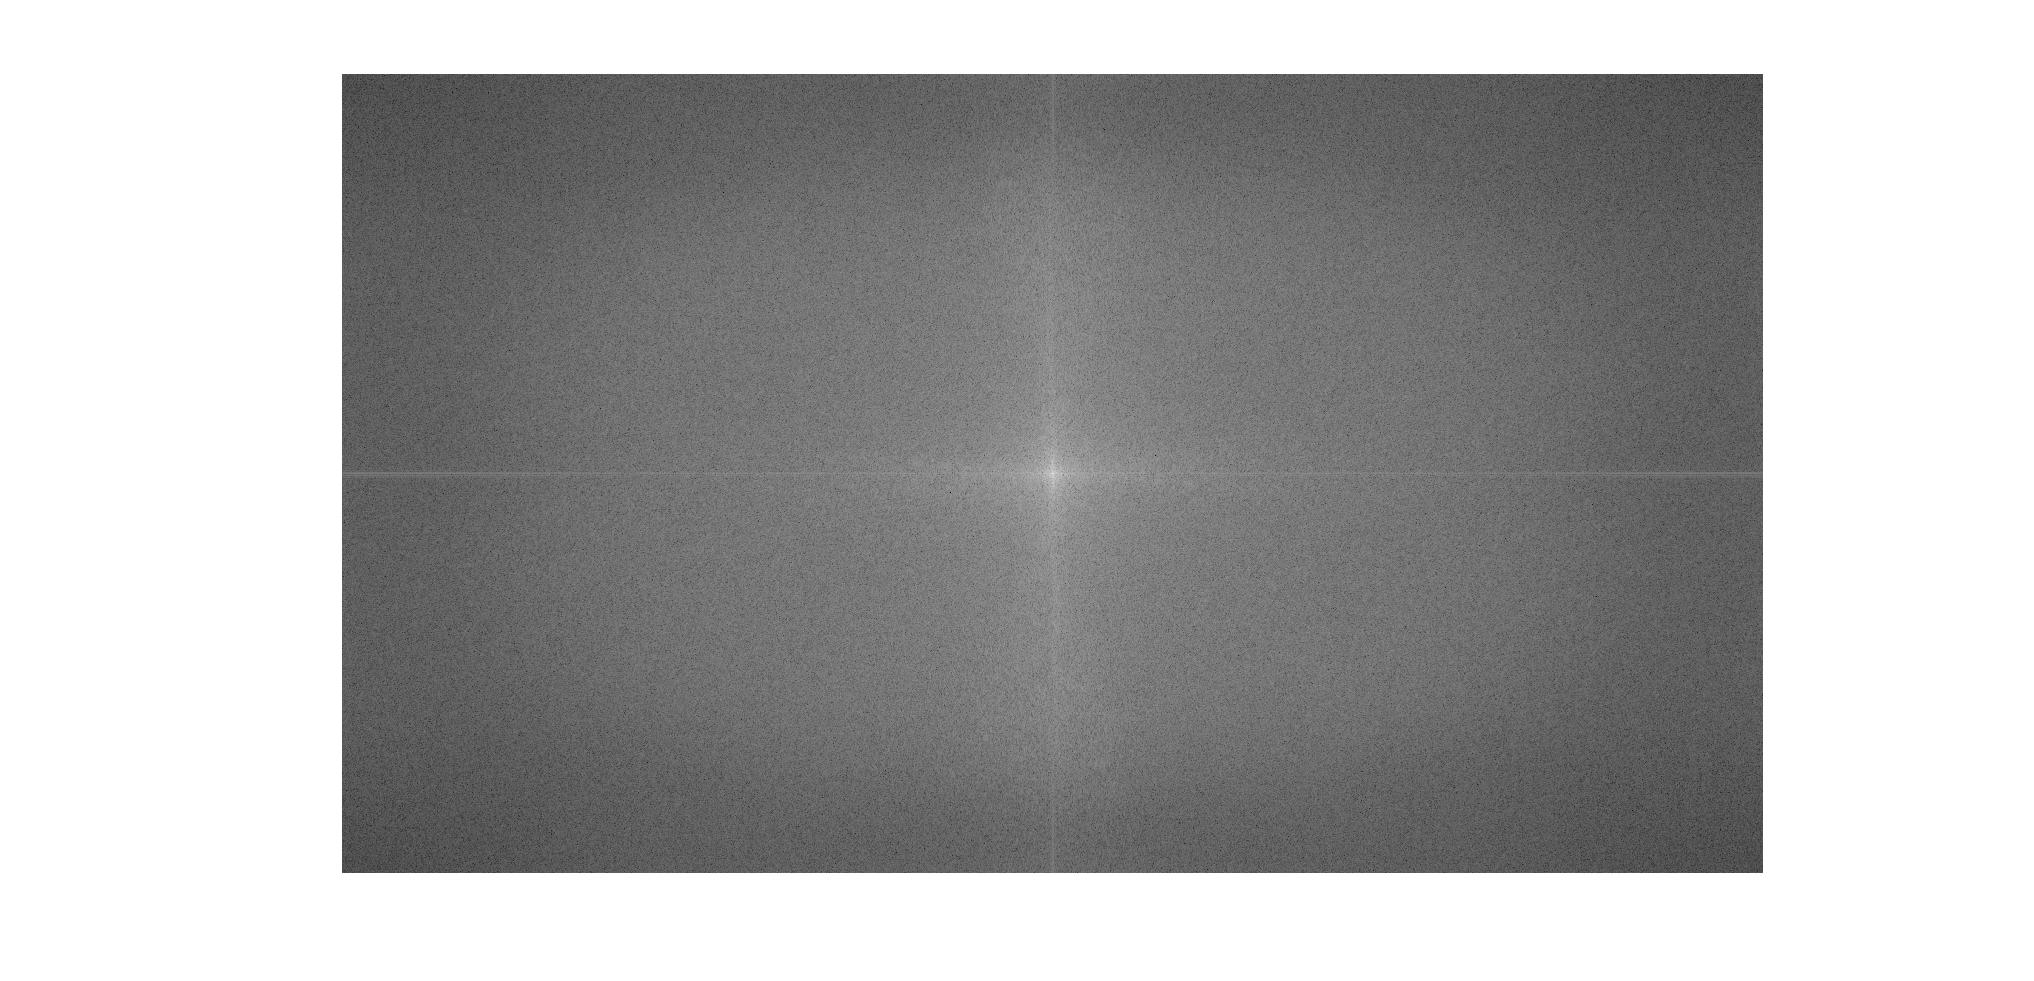
\includegraphics[width=\textwidth]{Images/FT_gray.jpg}
            \caption{تصویر خاکستری در حوزه فرکانس}
        \end{minipage}
        \begin{minipage}[b]{0.4\textwidth}
            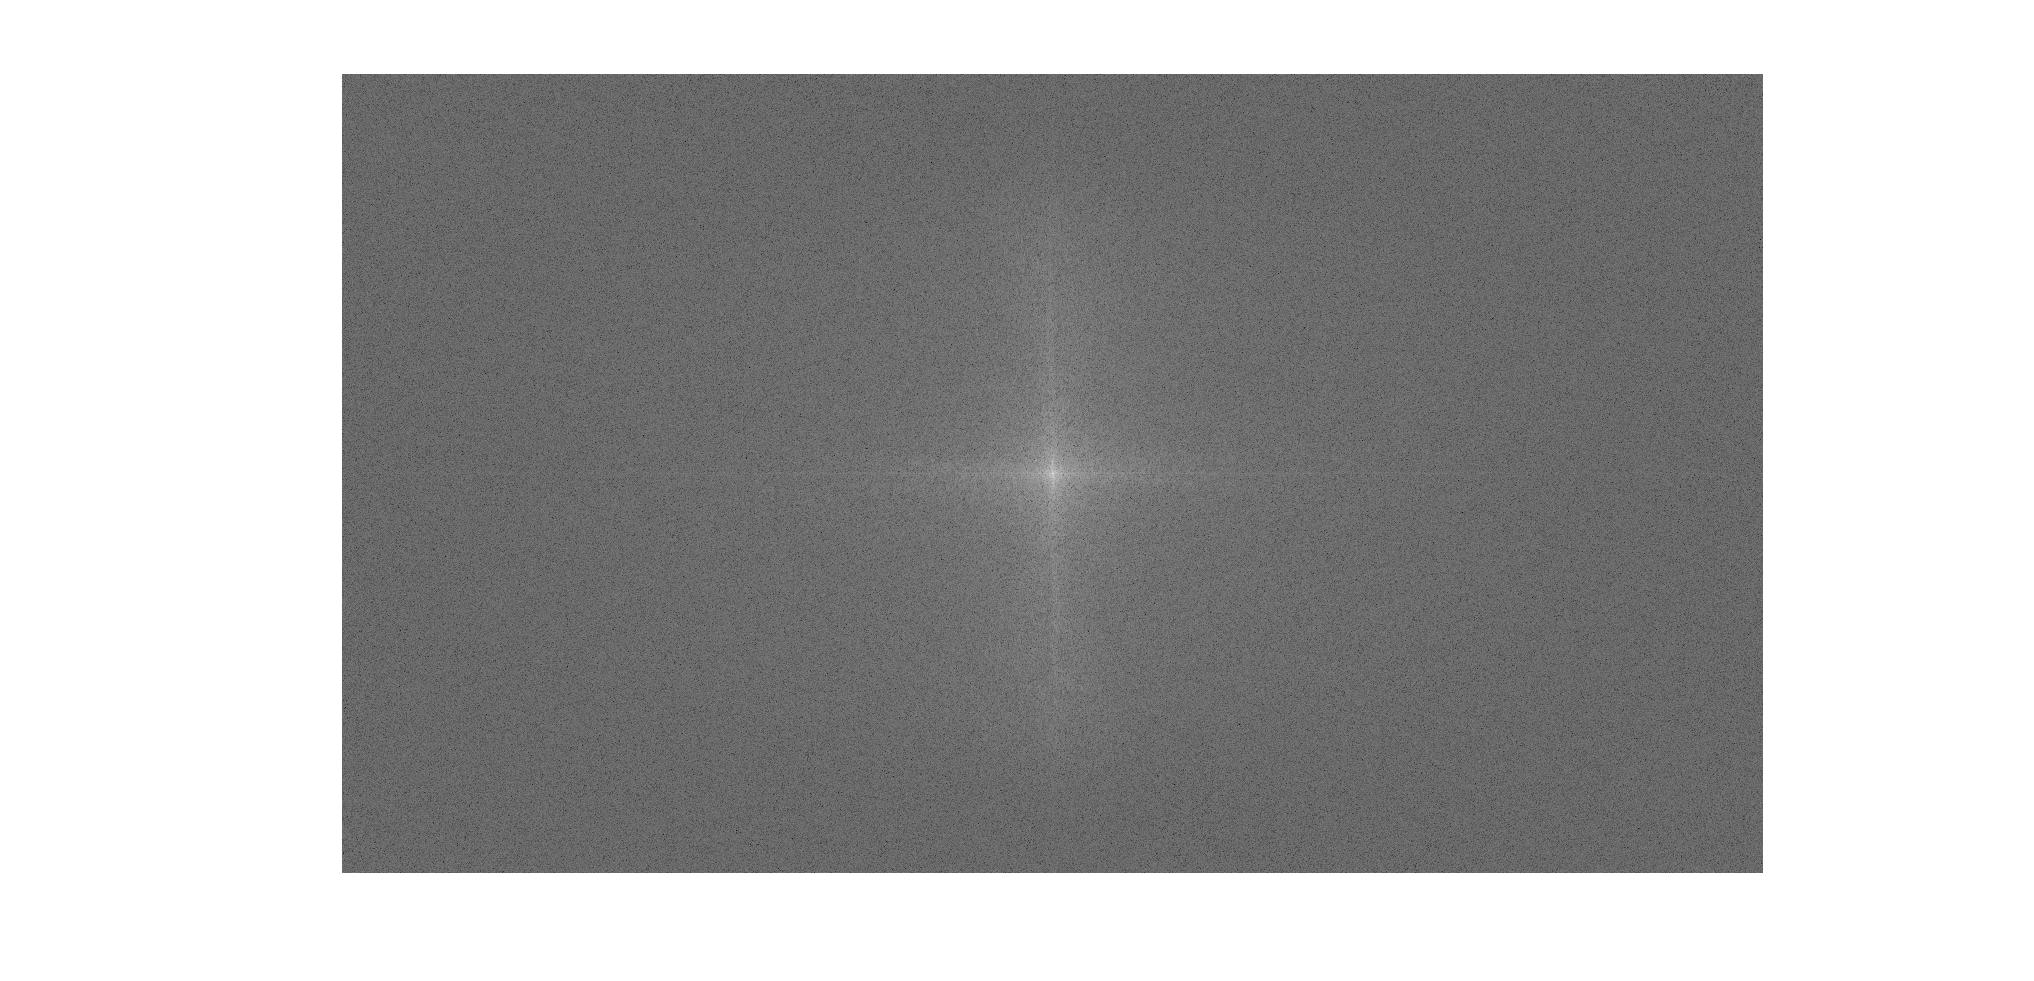
\includegraphics[width=\textwidth]{Images/FT_noisy.jpg}
            \caption{تصویر نویزی در حوزه فرکانس}
        \end{minipage}
    \end{figure}
    
    \begin{figure}[H]
        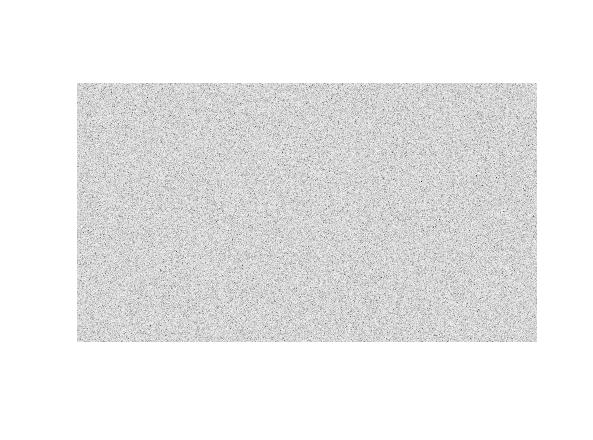
\includegraphics[width=6cm]{Images/FT_noise.jpg}
        \centering
        \caption{تصویر نویز در حوزه فرکانس}
    \end{figure}
    
    این تصاویر در واقع یک محور مختصات دو بعدی هستند که محور‌های آن شامل 
    \lr{Vertical frequency} و \lr{Horizontal frequency} است.
    مرکز تصویر مبدا این دستگاه مختصات است.
    مقدار روشنایی هر نقطه در این دستگاه مختصات، دامنه
    \lr{(Amplitude)} 
    فرکانس در آن نقطه است.
    
    در مرکز تصاویر که مبدا محور‌های فرکانس است و بزرگی فرکانس در آن نقطه کم است نقاط نورانی‌تر هستند و دامنه بیشتری دارند. این نشان می‌دهد اطلاعات تصویر در فرکانس‌های پایین یعنی مرکز تصویر ذخیره شده است.
    
    
    هر چه از مرکز دورتر می‌شویم و به اطراف می‌رویم بزرگی فرکانس‌ها افزایش می‌یابند ولی دامنه آن کمتر می‌شود و نقاط کم نورتر می‌شوند. این امر نشان می‌دهد اطلاعات کمی از تصویر در فرکانس‌های بالا ذخیره شده اند.
    
    با توجه به اینکه نویز اضافه شده از نوع گاوسی بوده و توزیع اطلاعات در آن یکسان است، یعنی نقاط سفید در تصویر نویز پخش هستند (شکل 9)، پس از اضافه شدن نویز تصویر فرکانسی روشن تر شده است (شکل 8)
    
    در واقع می‌توان گفت نقاط سفید در مرکز مربوط به تصویر اصلی بوده که دامنه بالا، فرکانس کم و اطلاعات زیاد دارد.
    نقاط سفید اطراف مربوط به نویز افزوده شده هست که فرکانس بالا، دامنه کم و اطلاعات کم دارد.
    
    بالاترین فرکانس‌ها در اطراف است که دامنه کمی دارد و کم نور است و پایین‌ترین فرکانس‌ها در مرکز وجود دارد که دامنه بالایی دارد و پر نور است.
    
    نکته: دستور شیفت باعث شده است که نقطه صفر فرکانس بر روی مرکز تصویر قرار گیرد.
}